\documentclass{article}

\usepackage{amsmath} % math stuff
\usepackage{amssymb} % math stuff
\usepackage{array} % equations and stuff
\usepackage{bm} % bold math
%\usepackage{booktabs} % extra table rule options
%\usepackage{caption} % suppressed table numbering; incompatible with revtex, and longtable, I think
\usepackage{comment} % comment environment
%\usepackage{enumitem} % customization of enumeration, itemize, and description
\usepackage[T1]{fontenc} % font encoding for special characters, must also use scalable font package
\usepackage[margin=0.8in]{geometry} % paper sizes and margins (but be careful not to mess up pre-defined pages)
\usepackage{graphicx} % for graphics
%\usepackage{helvet} % default font is the helvetica postscript font
\usepackage{layouts} % print units like widths
\usepackage{lipsum} % lorem ipsum filler text
\usepackage{lmodern} % scalable font?
\usepackage{longtable} % multi-page tables
\usepackage{makecell} % specify line-breaks in table cells
\usepackage{mathrsfs} % math script font
\usepackage{mhchem} % easier chemical formula
\usepackage{microtype} % allows disabling of ligatures
%\usepackage{newcent} % new century schoolbook font
\usepackage{nicefrac}
\usepackage{numprint} % print and format (large) numbers
\usepackage{parskip} % removes paragraph indentation, and adjusts paragraph skip, as well as list items
\usepackage{pdfpages} % add pdf files as pages
%\usepackage{setspace} % adjust text spacing and indents
\usepackage{siunitx} % decimal alignment
\usepackage{subfigure} % divided figures
%\usepackage{tabu} % extra table options
\usepackage{textcomp} % symbols
\usepackage{threeparttablex} % better footnotes with longtable
\usepackage{titling} % title placement
\usepackage{ulem} % strikethrough text
%\usepackage{url} % superceded by hyperref
\usepackage{verbatim} % verbatim environment
\usepackage{xcolor} % colors and color boxes
\usepackage{xspace} % commands that don't eat up white space
\usepackage{hyperref} % links and page setup; should always come last

\hypersetup{
 bookmarks=true,
 colorlinks=true,
 citecolor=blue,
 linkcolor=blue,
 urlcolor=blue,
 pdfstartview={XYZ null null 1.0} % default open view is 100%
}

\DisableLigatures[f,t]{encoding = T1} % disable ff, fi, fl, tt ligatures; without options, it also disables -- = endash
\renewcommand{\arraystretch}{1.0} % extra vertical (and horizontal?) space in tables

% define centered, left- and right-aligned columns with specified widths
\newcommand{\PreserveBackslash}[1]{\let\temp=\\#1\let\\=\temp}
\newcolumntype{C}[1]{>{\PreserveBackslash\centering}p{#1}}
\newcolumntype{L}[1]{>{\PreserveBackslash\raggedright}p{#1}}
\newcolumntype{R}[1]{>{\PreserveBackslash\raggedleft}p{#1}}

\begin{document}

\pagestyle{empty} % don't number pages

% custom title
\begin{center}
{\LARGE Classic Riddler}

\vspace{0.15in}

{\Large 9 April 2021}
\end{center}


\section*{Riddle:}

In Riddler City, all the streets are currently two-way streets.
But in an effort to make the metropolis friendlier for pedestrians and cyclists, the mayor has decreed that all streets should be one-way.
Meanwhile, the civil engineer overseeing this transition is not particularly invested in the project and will be randomly assigning every block of each street a random direction.

For your daily commute to work, you drive a car two blocks east and two blocks south, as shown in the diagram below.
What is the probability that, after each block is randomly assigned a one-way direction, there will still be a way for you to commute to work while staying within this two-by-two block region (i.e., sticking to the 12 streets you see in the diagram)?
Here is one such arrangement of one-way streets that lets you commute to work:

\vspace{0.1in}
\begin{center}
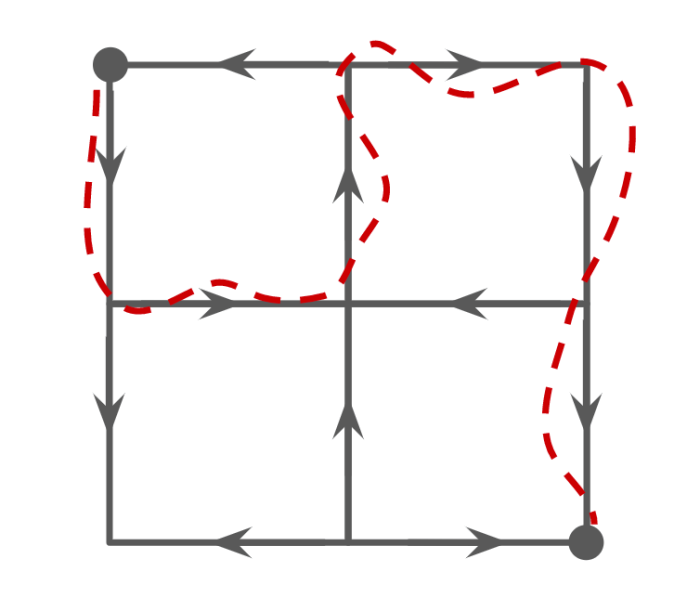
\includegraphics[width=3.5in]{streets.png}
\end{center}
\vspace{0.1in}

And no, you can't get out of your car to hop on a bike or walk.
I mean, you \textit{can}, but not in this puzzle.



\section*{Solution:}

Because there are 12 sections of road, there are $2^{12}=4096$ possible road arrangements.
This is too many to list all of them manually.
But I have decided to list and count them by grouping them into different classes of solutions.

There are two streets at the home corner, and at least one of these must be directed away from home (south or east).
Similarly, at least one of the two streets in the work corner must be directed to work (south or east).
Of the four possibilities for each, there are three valid arrangements.
I labeled these A, B, and C for the home corner arrangements and D, E, and F for the work corner arrangements.
I have shown my labels on the scanned page.

From here, I considered each of the 9 pairings of valid home and work arrangements, and then wrote out each of the classes of solutions using the remaining streets.
These can also be seen on the scanned page.
Many of the pairs had redundant solutions because of the symmetry of the problem, and so were not explicitly written out.
Specifically, I wrote out the A-E solutions, but A-F, B-D, and C-D would all have identical classes of solutions, so those weren't written out.
Similarly, B-E and C-F have the same solutions, as well as B-F and C-E.

For each class of solution, I wrote out the minimum arrangement of streets that led to a valid solution (while being distinct from previous classes).
For unlabeled streets, there are 2 possibilities that don't change the solution.
So I simply counted the unlabeled streets to get the number of solutions in each class.
For example (in the A-D pairing), for the class with both top streets pointing east and both right streets pointing south, there are 6 unlabeled streets, leading to $2^{6}=64$ solutions in that class.

In total, there are 193 solutions in the A-D pairing, 139 solutions in the A-E (and A-F, B-D, C-D) pairing, 81 solutions in the B-E (and C-F) pairing, and 112 solutions in the B-F (and C-E) pairing.
That gives a total of 1,135 solutions.
I am certain that the classes I wrote out are all distinct, and that this answer does not double count any solutions, but I am not totally certain that this is an exhaustive answer. But the best answer I have is
\fcolorbox{red}{white}{$\bm{{\nicefrac{1135}{4096}\approx27.7\%}}$}\,.

\includepdf{scan.pdf}


\end{document}